\documentclass[a4j,10pt]{jsarticle}
\usepackage{layout,url,resume}
\usepackage[dvipdfmx]{graphicx}
\pagestyle{empty}

\begin{document}
%\layout

\title{スマートフォンのブラウザで視聴中のWebページ・動画の視聴位置を保存・復旧するしおりアプリ}

% 和文著者名
\author{
    Arch B3 新真虎(masatora) \thanks{慶應義塾大学環境情報学部}
    \and
    Adviser: 松谷健史(macchan) \thanks{慶應義塾大学大学院 政策・メディアメディア研究科特任講師}
}

\maketitle
\thispagestyle{empty}

\section{背景}
スマートフォンでネットサーフィンをしているとき、読んでいる途中のページや動画をブックマークしたいというニーズがある。
そうしたニーズに対応するブックマークアプリはすでに存在する\cite{Pocket}\cite{instapaper}。

しかし、既存のブックマークアプリには以下の問題がある。
\begin{enumerate}
\item 保存したWebページのスクロール位置がわからなくなる
\item 保存した動画の再生位置(何分何秒まで見ていた・何分何秒が面白かった)がわからなくなる
\end{enumerate}

その結果、Webページや動画の視聴を再開したり、誰かに共有するたびに、
どこまで読んでいたか・見ていたかを探す時間が無駄になってしまう。

%---------------------------------------------

\section{目的}
上記の問題を解決するため、スマートフォンで見ているWebページや動画をどこまで読んでいたか・
どこまで見ていたかという情報とともに保存し、復旧できるようにすることを目指す。

\section{目標}
Webページおよび動画のスクロール位置や再生位置を保存・復旧することのできる
iOSアプリケーションを開発する\cite{shiori-web-for-safari}。

\section{先行研究}
既存のブックマークアプリケーションとしては、
Safariが標準で提供しているリーディングリスト、
Pocket\cite{Pocket} 、instapaper\cite{instapaper}等が存在している。それらのアプリケーションの
機能を表\ref{table1}にまとめた。

\begin{table}[t]
    \caption{}
    \label{table1}
    \begin{center}
        \scalebox{0.7}{
        \begin{tabular}
        {|p{4cm}|p{2.5cm}|p{2.5cm}|p{2.5cm}|}
        \hline
        & safariのリーディングリスト & Pocket\cite{Pocket} & instapaper\cite{instapaper} \\
        \hline
        Webページをブックマークする機能 & ◯ & ◯ & ◯ \\
        \hline
        動画をブックマークする機能 & ◯ & ◯ & ◯ \\
        \hline
        ブックマークしたWebページのスクロール位置を復旧する機能 & × & × & × \\
        \hline
        ブックマークした動画の再生位置を復旧する機能 & × & × & × \\
        \hline
        \end{tabular}
        }
    \end{center}
\end{table}

\section{アプローチ}
\subsection{ブックマークしたWebページのスクロール位置を復旧する機能}
ユーザーが開いているWebページのスクロール位置(縦・横)を取得する。
ユーザーがWebページをブックマークしたとき、そのWebページのURLとともに取得した
スクロール位置をアプリ内に保存する。
そして、アプリ内でブックマークしたWebページを開いたタイミングで、
取得した位置にスクロールする。

\subsection{ブックマークした動画の再生位置を復旧する機能}
ユーザーが視聴している動画の再生位置(秒単位)を取得する。
ユーザーが動画をブックマークしたとき、その動画のURLとともに取得した
再生位置をアプリ内に保存する。
そして、アプリ内でブックマークした動画を開いたタイミングで、
取得したURLから動画サイトの種類を判別する。
動画を開く際に、クエリパラメータとして動画再生位置を指定することで、
再生位置を復旧する。

\section{環境}
\begin{itemize}
\item Xcode12
\item Swift5
\item ECMAScript 2015
\end{itemize}

\section{実装}
\subsection{ユーザーがWebページを保存するまでの手順}
ユーザーがこのアプリケーションを使用してWebページ・動画を保存し、
復旧するまでの主な手順を以下に示した。
\begin{enumerate}
\item SafariでWebページや動画を視聴している(図\ref{fig:one})
\item 共有ボタンをタップ(図\ref{fig:one})
\item 「Shiori」ボタンをタップして保存する(図\ref{fig:two})
\item アプリを開くと、視聴していたWebページ・動画が保存されている(図\ref{fig:two})
\item 保存したWebページ・動画をタップすると、スクロール位置・再生位置が復旧された状態でWebページ・動画が開かれる(図\ref{fig:two})
\end{enumerate}

\begin{figure}[htbp]
    \begin{minipage}{0.5\hsize}
        \begin{center}
        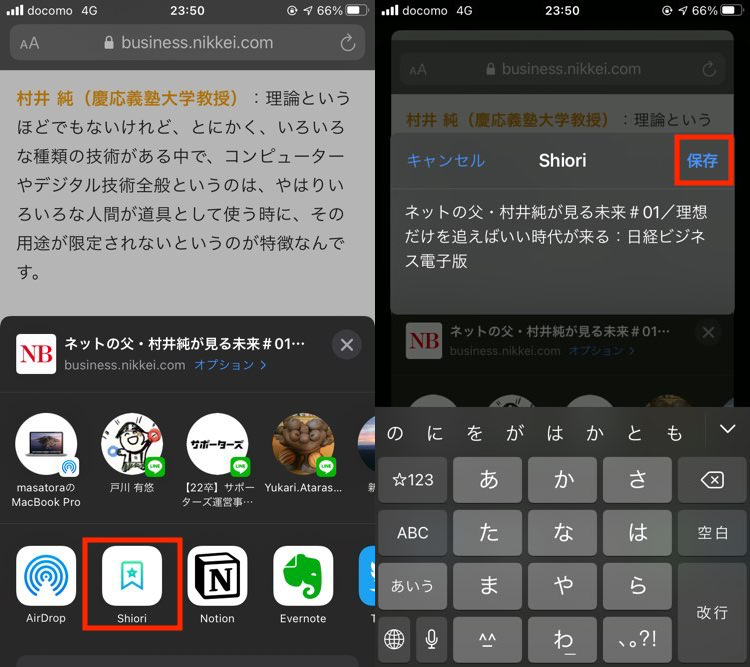
\includegraphics[width=70mm]{../assets/scroll_position/scroll_position1.png}
        \end{center}
        \caption{}
        \label{fig:one}
    \end{minipage}
    \begin{minipage}{0.5\hsize}
        \begin{center}
        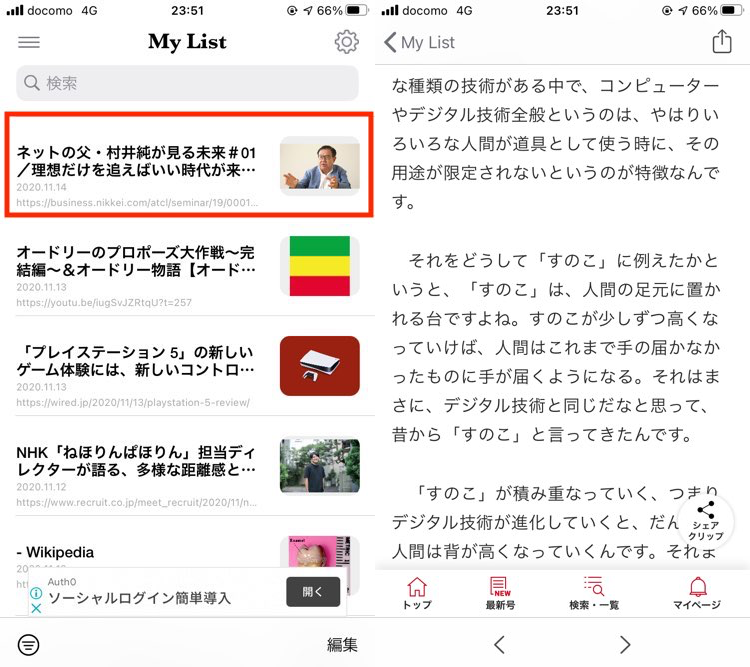
\includegraphics[width=70mm]{../assets/scroll_position/scroll_position2.png}
        \end{center}
        \caption{}
        \label{fig:two}
    \end{minipage}
\end{figure}

\subsection{プログラム間でのデータフロー}
上記の機能を実現するため、Appleが提供するApp Extension\cite{App-Extension}の
一種であるShare Extension\cite{Share-Extension}という機能を利用する。
Share Extensionとは、iPhoneで開いているWebページや動画を
任意のアプリケーションに保存できる機能である。
Share Extensionを利用してアプリにWebページや動画を保存するタイミングで
Javascriptコードを実行し、以下の二つのデータを取得する。
\begin{itemize}
\item スクロール位置
\item 動画の再生時間
\end{itemize}

そして、取得したデータをWebページや動画のメタデータとして保存する。
ユーザーが保存したWebページや動画をクリックすると、アプリケーション内部で
ブラウザを開き、スクロール位置や再生位置を復旧させた状態でWebページや動画を開く。


\section{評価}
評価のために、開発したアプリケーションが以下の2つの機能を実現できていることを確認する。
\begin{enumerate}
\item 保存したWebページのスクロール位置が復旧できること
\item 保存した動画の再生位置が復旧できること
\end{enumerate}

評価の方法として、実際に任意のWebページ・動画を途中までスクロール・再生した上で
アプリケーションに保存する。保存されたWebページ・動画をアプリケーション内で開き、
保存したときのスクロール位置・再生位置が復旧するかどうか検証する。

検証には、以下のWebページ・動画を使用した。
\begin{enumerate}
\item Webページ: ネットの父・村井純が見る未来#01/理想だけを追えばいい時代が来る\cite{murai-web-page}
\item 動画: 「インターネット文明」村井純\cite{murai-video}
\end{enumerate}

\section{結果}
\subsection{実現できたこと}
評価の結果実現できた機能を、先行研究との比較とともに表\ref{table2}にまとめた。
\begin{table}[t]
    \caption{}
    \label{table2}
    \begin{center}
        \scalebox{0.6}{
        \begin{tabular}
        {|p{3cm}|p{2cm}|p{2cm}|p{2cm}|p{2cm}|}
        \hline
        & Shiori web & safariのリーディングリスト & Pocket\cite{Pocket} & instapaper\cite{instapaper} \\
        \hline
        ブックマークしたWebページのスクロール位置を復旧する機能(縦スクロール) & ◯ & × & × & × \\
        \hline
        ブックマークしたWebページのスクロール位置を復旧する機能(横スクロール) & ◯ & × & × & × \\
        \hline
        ブックマークした動画の再生位置を復旧する機能 & △ & × & × & × \\
        \hline
        \end{tabular}
        }
    \end{center}
\end{table}

\subsection{実現できていないこと}
一方、実現できていない点とその原因は以下である。
\subsubsection{一部対応できていない動画サイトが存在する}
原因: 再生位置を指定して途中から動画を再生する、という機能を提供していない動画サイトがあるため。

\subsubsection{埋め込み動画に対応できていない}
原因: URLから動画サイトを判定し、各動画サイトがそれぞれ公開しているAPIのクエリパラメータの形式に合わせてリクエストを送ることで再生位置を復旧する機能を実現している。そのため、URLから動画の元サイトを判定できない埋め込み動画では、再生位置を復旧する機能が動作しない。

\subsubsection{動画再生位置は秒単位にしか対応していない}
原因: 再生位置を秒単位で取得しているため、それより細かい単位での動画再生位置復旧はできない。

\bibliographystyle{junsrt}
\bibliography{resume}

\end{document}
% end of file
